% Options for packages loaded elsewhere
\PassOptionsToPackage{unicode}{hyperref}
\PassOptionsToPackage{hyphens}{url}
%
\documentclass[
]{article}
\usepackage{lmodern}
\usepackage{amssymb,amsmath}
\usepackage{ifxetex,ifluatex}
\ifnum 0\ifxetex 1\fi\ifluatex 1\fi=0 % if pdftex
  \usepackage[T1]{fontenc}
  \usepackage[utf8]{inputenc}
  \usepackage{textcomp} % provide euro and other symbols
\else % if luatex or xetex
  \usepackage{unicode-math}
  \defaultfontfeatures{Scale=MatchLowercase}
  \defaultfontfeatures[\rmfamily]{Ligatures=TeX,Scale=1}
\fi
% Use upquote if available, for straight quotes in verbatim environments
\IfFileExists{upquote.sty}{\usepackage{upquote}}{}
\IfFileExists{microtype.sty}{% use microtype if available
  \usepackage[]{microtype}
  \UseMicrotypeSet[protrusion]{basicmath} % disable protrusion for tt fonts
}{}
\makeatletter
\@ifundefined{KOMAClassName}{% if non-KOMA class
  \IfFileExists{parskip.sty}{%
    \usepackage{parskip}
  }{% else
    \setlength{\parindent}{0pt}
    \setlength{\parskip}{6pt plus 2pt minus 1pt}}
}{% if KOMA class
  \KOMAoptions{parskip=half}}
\makeatother
\usepackage{xcolor}
\IfFileExists{xurl.sty}{\usepackage{xurl}}{} % add URL line breaks if available
\IfFileExists{bookmark.sty}{\usepackage{bookmark}}{\usepackage{hyperref}}
\hypersetup{
  pdftitle={GWAS Visualization in R},
  pdfauthor={Keith Mitchel, UC Davis Bioinformatics Core},
  hidelinks,
  pdfcreator={LaTeX via pandoc}}
\urlstyle{same} % disable monospaced font for URLs
\usepackage[margin=1in]{geometry}
\usepackage{color}
\usepackage{fancyvrb}
\newcommand{\VerbBar}{|}
\newcommand{\VERB}{\Verb[commandchars=\\\{\}]}
\DefineVerbatimEnvironment{Highlighting}{Verbatim}{commandchars=\\\{\}}
% Add ',fontsize=\small' for more characters per line
\usepackage{framed}
\definecolor{shadecolor}{RGB}{248,248,248}
\newenvironment{Shaded}{\begin{snugshade}}{\end{snugshade}}
\newcommand{\AlertTok}[1]{\textcolor[rgb]{0.94,0.16,0.16}{#1}}
\newcommand{\AnnotationTok}[1]{\textcolor[rgb]{0.56,0.35,0.01}{\textbf{\textit{#1}}}}
\newcommand{\AttributeTok}[1]{\textcolor[rgb]{0.77,0.63,0.00}{#1}}
\newcommand{\BaseNTok}[1]{\textcolor[rgb]{0.00,0.00,0.81}{#1}}
\newcommand{\BuiltInTok}[1]{#1}
\newcommand{\CharTok}[1]{\textcolor[rgb]{0.31,0.60,0.02}{#1}}
\newcommand{\CommentTok}[1]{\textcolor[rgb]{0.56,0.35,0.01}{\textit{#1}}}
\newcommand{\CommentVarTok}[1]{\textcolor[rgb]{0.56,0.35,0.01}{\textbf{\textit{#1}}}}
\newcommand{\ConstantTok}[1]{\textcolor[rgb]{0.00,0.00,0.00}{#1}}
\newcommand{\ControlFlowTok}[1]{\textcolor[rgb]{0.13,0.29,0.53}{\textbf{#1}}}
\newcommand{\DataTypeTok}[1]{\textcolor[rgb]{0.13,0.29,0.53}{#1}}
\newcommand{\DecValTok}[1]{\textcolor[rgb]{0.00,0.00,0.81}{#1}}
\newcommand{\DocumentationTok}[1]{\textcolor[rgb]{0.56,0.35,0.01}{\textbf{\textit{#1}}}}
\newcommand{\ErrorTok}[1]{\textcolor[rgb]{0.64,0.00,0.00}{\textbf{#1}}}
\newcommand{\ExtensionTok}[1]{#1}
\newcommand{\FloatTok}[1]{\textcolor[rgb]{0.00,0.00,0.81}{#1}}
\newcommand{\FunctionTok}[1]{\textcolor[rgb]{0.00,0.00,0.00}{#1}}
\newcommand{\ImportTok}[1]{#1}
\newcommand{\InformationTok}[1]{\textcolor[rgb]{0.56,0.35,0.01}{\textbf{\textit{#1}}}}
\newcommand{\KeywordTok}[1]{\textcolor[rgb]{0.13,0.29,0.53}{\textbf{#1}}}
\newcommand{\NormalTok}[1]{#1}
\newcommand{\OperatorTok}[1]{\textcolor[rgb]{0.81,0.36,0.00}{\textbf{#1}}}
\newcommand{\OtherTok}[1]{\textcolor[rgb]{0.56,0.35,0.01}{#1}}
\newcommand{\PreprocessorTok}[1]{\textcolor[rgb]{0.56,0.35,0.01}{\textit{#1}}}
\newcommand{\RegionMarkerTok}[1]{#1}
\newcommand{\SpecialCharTok}[1]{\textcolor[rgb]{0.00,0.00,0.00}{#1}}
\newcommand{\SpecialStringTok}[1]{\textcolor[rgb]{0.31,0.60,0.02}{#1}}
\newcommand{\StringTok}[1]{\textcolor[rgb]{0.31,0.60,0.02}{#1}}
\newcommand{\VariableTok}[1]{\textcolor[rgb]{0.00,0.00,0.00}{#1}}
\newcommand{\VerbatimStringTok}[1]{\textcolor[rgb]{0.31,0.60,0.02}{#1}}
\newcommand{\WarningTok}[1]{\textcolor[rgb]{0.56,0.35,0.01}{\textbf{\textit{#1}}}}
\usepackage{graphicx,grffile}
\makeatletter
\def\maxwidth{\ifdim\Gin@nat@width>\linewidth\linewidth\else\Gin@nat@width\fi}
\def\maxheight{\ifdim\Gin@nat@height>\textheight\textheight\else\Gin@nat@height\fi}
\makeatother
% Scale images if necessary, so that they will not overflow the page
% margins by default, and it is still possible to overwrite the defaults
% using explicit options in \includegraphics[width, height, ...]{}
\setkeys{Gin}{width=\maxwidth,height=\maxheight,keepaspectratio}
% Set default figure placement to htbp
\makeatletter
\def\fps@figure{htbp}
\makeatother
\setlength{\emergencystretch}{3em} % prevent overfull lines
\providecommand{\tightlist}{%
  \setlength{\itemsep}{0pt}\setlength{\parskip}{0pt}}
\setcounter{secnumdepth}{-\maxdimen} % remove section numbering

\title{GWAS Visualization in R}
\author{Keith Mitchel, UC Davis Bioinformatics Core}
\date{7/7/2021}

\begin{document}
\maketitle

{
\setcounter{tocdepth}{2}
\tableofcontents
}
\hypertarget{we-will-need-to-get-the-tdt-results-for-the-data}{%
\section{We will need to get the tdt results for the
data}\label{we-will-need-to-get-the-tdt-results-for-the-data}}

\hypertarget{todo-auto-install-chunk-not-sure-i-remember-how-we-do-this}{%
\section{TODO auto install chunk? Not sure I remember how we do
this}\label{todo-auto-install-chunk-not-sure-i-remember-how-we-do-this}}

\begin{itemize}
\tightlist
\item
  explain packages as well.
\end{itemize}

\begin{Shaded}
\begin{Highlighting}[]
\CommentTok{#install.packages("qqman")}
\CommentTok{#install.packages("CMplot")}
\end{Highlighting}
\end{Shaded}

\begin{Shaded}
\begin{Highlighting}[]
\KeywordTok{library}\NormalTok{(qqman)}
\KeywordTok{library}\NormalTok{(dplyr)}
\end{Highlighting}
\end{Shaded}

For a comparison, a sample dataset is provided in order to show what all
chromosomes would look like. We will create some visualization with this
as well.

\begin{Shaded}
\begin{Highlighting}[]
\KeywordTok{head}\NormalTok{(gwasResults)}
\end{Highlighting}
\end{Shaded}

\begin{verbatim}
##   SNP CHR BP         P
## 1 rs1   1  1 0.9148060
## 2 rs2   1  2 0.9370754
## 3 rs3   1  3 0.2861395
## 4 rs4   1  4 0.8304476
## 5 rs5   1  5 0.6417455
## 6 rs6   1  6 0.5190959
\end{verbatim}

Lets read in the TDT results - The adjusted file is a bit smaller here
since the NA values cannot be adjusted and are ommitted. So lets merge
and only keep values that exist in the adjusted file, but lets add the
frequency or MAF

\begin{Shaded}
\begin{Highlighting}[]
\NormalTok{tdtfrq <-}\StringTok{ }\KeywordTok{read.csv}\NormalTok{(}\StringTok{"../tdtfrq.csv"}\NormalTok{)}
\KeywordTok{head}\NormalTok{(tdtfrq)}
\end{Highlighting}
\end{Shaded}

\begin{verbatim}
##   CHR     SNP A1 A2      MAF NCHROBS
## 1  21 5034209  A  G 0.003571     280
## 2  21 5034244  T  C 0.007042     284
## 3  21 5063575  T  C 0.003497     286
## 4  21 5063806  T  C 0.003448     290
## 5  21 5063842  A  G 0.010420     288
## 6  21 5089937  C  T 0.017240     290
\end{verbatim}

\begin{Shaded}
\begin{Highlighting}[]
\NormalTok{tdtadj <-}\StringTok{ }\KeywordTok{read.csv}\NormalTok{(}\StringTok{"../tdtadj.csv"}\NormalTok{, }\DataTypeTok{row.names=}\OtherTok{NULL}\NormalTok{)}
\KeywordTok{head}\NormalTok{(tdtadj)}
\end{Highlighting}
\end{Shaded}

\begin{verbatim}
##   CHR     SNP     UNADJ       GC BONF HOLM SIDAK_SS SIDAK_SD FDR_BH FDR_BY
## 1  21 7946755 6.334e-05 0.006911    1    1   0.9949   0.9949 0.3764      1
## 2  21 7946763 6.334e-05 0.006911    1    1   0.9949   0.9949 0.3764      1
## 3  21 7946728 1.075e-04 0.008914    1    1   0.9999   0.9999 0.3764      1
## 4  21 7946741 1.075e-04 0.008914    1    1   0.9999   0.9999 0.3764      1
## 5  21 7946744 1.075e-04 0.008914    1    1   0.9999   0.9999 0.3764      1
## 6  21 7946776 1.828e-04 0.011520    1    1   1.0000   1.0000 0.3764      1
\end{verbatim}

Lets merge our frequences with the TDT results.

\begin{Shaded}
\begin{Highlighting}[]
\NormalTok{cleantdt <-}\StringTok{ }\KeywordTok{merge}\NormalTok{(tdtfrq , tdtadj, }\DataTypeTok{by=}\KeywordTok{c}\NormalTok{(}\StringTok{"CHR"}\NormalTok{,}\StringTok{"SNP"}\NormalTok{))}
\KeywordTok{head}\NormalTok{(cleantdt)}
\end{Highlighting}
\end{Shaded}

\begin{verbatim}
##   CHR      SNP A1 A2      MAF NCHROBS  UNADJ     GC BONF HOLM SIDAK_SS
## 1  21 10000132 AT  A 0.003448     290 0.3173 0.4995    1    1        1
## 2  21 10000176 AT  A 0.003448     290 0.3173 0.4995    1    1        1
## 3  21 10000297  A  G 0.006897     290 0.3173 0.4995    1    1        1
## 4  21 10000415  G  T 0.003448     290 1.0000 1.0000    1    1        1
## 5  21 10000434  A  G 0.003448     290 0.3173 0.4995    1    1        1
## 6  21 10000714  A  G 0.489600     288 0.7003 0.7949    1    1        1
##   SIDAK_SD FDR_BH FDR_BY
## 1        1 0.3764      1
## 2        1 0.3764      1
## 3        1 0.3764      1
## 4        1 1.0000      1
## 5        1 0.3764      1
## 6        1 0.7868      1
\end{verbatim}

Lets read in the annotation information

\begin{Shaded}
\begin{Highlighting}[]
\NormalTok{anno <-}\StringTok{ }\KeywordTok{read.csv}\NormalTok{(}\StringTok{'~/Downloads/query.output.genome_summary.csv'}\NormalTok{)}
\KeywordTok{head}\NormalTok{(anno)}
\end{Highlighting}
\end{Shaded}

\begin{verbatim}
##   Chr   Start     End Ref Alt Func.refGene     Gene.refGene
## 1  21 5034209 5034209   G   A     intronic           ICOSLG
## 2  21 5034244 5034244   C   T     intronic           ICOSLG
## 3  21 5063575 5063575   C   T   intergenic ICOSLG;LINC01678
## 4  21 5063806 5063806   C   T   intergenic ICOSLG;LINC01678
## 5  21 5063842 5063842   G   A   intergenic ICOSLG;LINC01678
## 6  21 5089937 5089937   T   C   intergenic ICOSLG;LINC01678
##      GeneDetail.refGene ExonicFunc.refGene AAChange.refGene X1000G_ALL
## 1                                                                     
## 2                                                                     
## 3 dist=22907;dist=38485                                               
## 4 dist=23138;dist=38254                                               
## 5 dist=23174;dist=38218                                               
## 6 dist=49269;dist=12123                                               
##   X1000G_AFR X1000G_AMR X1000G_EAS X1000G_EUR X1000G_SAS ExAC_Freq ExAC_AFR
## 1                                                                          
## 2                                                                          
## 3                                                                          
## 4                                                                          
## 5                                                                          
## 6                                                                          
##   ExAC_AMR ExAC_EAS ExAC_FIN ExAC_NFE ExAC_OTH ExAC_SAS ESP6500si_ALL
## 1                                                                    
## 2                                                                    
## 3                                                                    
## 4                                                                    
## 5                                                                    
## 6                                                                    
##   ESP6500si_AA ESP6500si_EA CG46 NCI60 dbSNP COSMIC_ID COSMIC_DIS ClinVar_SIG
## 1                                                                            
## 2                                                                            
## 3                                                                            
## 4                                                                            
## 5                                                                            
## 6                                                                            
##   ClinVar_DIS ClinVar_ID ClinVar_DB ClinVar_DBID GWAS_DIS GWAS_OR GWAS_BETA
## 1                                                                          
## 2                                                                          
## 3                                                                          
## 4                                                                          
## 5                                                                          
## 6                                                                          
##   GWAS_PUBMED GWAS_SNP GWAS_P SIFT_score SIFT_converted_rankscore SIFT_pred
## 1                                                                          
## 2                                                                          
## 3                                                                          
## 4                                                                          
## 5                                                                          
## 6                                                                          
##   Polyphen2_HDIV_score Polyphen2_HDIV_rankscore Polyphen2_HDIV_pred
## 1                                                                  
## 2                                                                  
## 3                                                                  
## 4                                                                  
## 5                                                                  
## 6                                                                  
##   Polyphen2_HVAR_score Polyphen2_HVAR_rankscore Polyphen2_HVAR_pred LRT_score
## 1                                                                            
## 2                                                                            
## 3                                                                            
## 4                                                                            
## 5                                                                            
## 6                                                                            
##   LRT_converted_rankscore LRT_pred MutationTaster_score
## 1                                                      
## 2                                                      
## 3                                                      
## 4                                                      
## 5                                                      
## 6                                                      
##   MutationTaster_converted_rankscore MutationTaster_pred
## 1                                                       
## 2                                                       
## 3                                                       
## 4                                                       
## 5                                                       
## 6                                                       
##   MutationAssessor_score MutationAssessor_score_rankscore
## 1                                                        
## 2                                                        
## 3                                                        
## 4                                                        
## 5                                                        
## 6                                                        
##   MutationAssessor_pred FATHMM_score FATHMM_converted_rankscore FATHMM_pred
## 1                                                                          
## 2                                                                          
## 3                                                                          
## 4                                                                          
## 5                                                                          
## 6                                                                          
##   PROVEAN_score PROVEAN_converted_rankscore PROVEAN_pred VEST3_score
## 1                                                                   
## 2                                                                   
## 3                                                                   
## 4                                                                   
## 5                                                                   
## 6                                                                   
##   VEST3_rankscore MetaSVM_score MetaSVM_rankscore MetaSVM_pred MetaLR_score
## 1                                                                          
## 2                                                                          
## 3                                                                          
## 4                                                                          
## 5                                                                          
## 6                                                                          
##   MetaLR_rankscore MetaLR_pred M.CAP_score M.CAP_rankscore M.CAP_pred
## 1                                                                    
## 2                                                                    
## 3                                                                    
## 4                                                                    
## 5                                                                    
## 6                                                                    
##   CADD_raw CADD_raw_rankscore CADD_phred DANN_score DANN_rankscore
## 1                                                                 
## 2                                                                 
## 3                                                                 
## 4                                                                 
## 5                                                                 
## 6                                                                 
##   fathmm.MKL_coding_score fathmm.MKL_coding_rankscore fathmm.MKL_coding_pred
## 1                                                                           
## 2                                                                           
## 3                                                                           
## 4                                                                           
## 5                                                                           
## 6                                                                           
##   Eigen_coding_or_noncoding Eigen.raw Eigen.PC.raw GenoCanyon_score
## 1                                                                  
## 2                                                                  
## 3                                                                  
## 4                                                                  
## 5                                                                  
## 6                                                                  
##   GenoCanyon_score_rankscore integrated_fitCons_score
## 1                                                    
## 2                                                    
## 3                                                    
## 4                                                    
## 5                                                    
## 6                                                    
##   integrated_fitCons_score_rankscore integrated_confidence_value GERP.._RS
## 1                                                                         
## 2                                                                         
## 3                                                                         
## 4                                                                         
## 5                                                                         
## 6                                                                         
##   GERP.._RS_rankscore phyloP100way_vertebrate
## 1                                            
## 2                                            
## 3                                            
## 4                                            
## 5                                            
## 6                                            
##   phyloP100way_vertebrate_rankscore phyloP20way_mammalian
## 1                                                        
## 2                                                        
## 3                                                        
## 4                                                        
## 5                                                        
## 6                                                        
##   phyloP20way_mammalian_rankscore phastCons100way_vertebrate
## 1                                                           
## 2                                                           
## 3                                                           
## 4                                                           
## 5                                                           
## 6                                                           
##   phastCons100way_vertebrate_rankscore phastCons20way_mammalian
## 1                                                              
## 2                                                              
## 3                                                              
## 4                                                              
## 5                                                              
## 6                                                              
##   phastCons20way_mammalian_rankscore SiPhy_29way_logOdds
## 1                                                       
## 2                                                       
## 3                                                       
## 4                                                       
## 5                                                       
## 6                                                       
##   SiPhy_29way_logOdds_rankscore Interpro_domain GTEx_V6_gene GTEx_V6_tissue
## 1                                                                          
## 2                                                                          
## 3                                                                          
## 4                                                                          
## 5                                                                          
## 6                                                                          
##   gnomAD_exome_ALL gnomAD_exome_AFR gnomAD_exome_AMR gnomAD_exome_ASJ
## 1                                                                    
## 2                                                                    
## 3                                                                    
## 4                                                                    
## 5                                                                    
## 6                                                                    
##   gnomAD_exome_EAS gnomAD_exome_FIN gnomAD_exome_NFE gnomAD_exome_OTH
## 1                                                                    
## 2                                                                    
## 3                                                                    
## 4                                                                    
## 5                                                                    
## 6                                                                    
##   gnomAD_exome_SAS gnomAD_genome_ALL gnomAD_genome_AFR gnomAD_genome_AMR
## 1                                                                       
## 2                                                                       
## 3                                                                       
## 4                                                                       
## 5                                                                       
## 6                                                                       
##   gnomAD_genome_ASJ gnomAD_genome_EAS gnomAD_genome_FIN gnomAD_genome_NFE
## 1                                                                        
## 2                                                                        
## 3                                                                        
## 4                                                                        
## 5                                                                        
## 6                                                                        
##   gnomAD_genome_OTH Otherinfo Otherinfo.1
## 1                         hom           .
## 2                         hom           .
## 3                         hom           .
## 4                         hom           .
## 5                         hom           .
## 6                         hom           .
\end{verbatim}

There seem to be some NA values produced by plink for TDT.. why might
this be?

\begin{Shaded}
\begin{Highlighting}[]
\NormalTok{final <-}\StringTok{ }\KeywordTok{merge}\NormalTok{(cleantdt, anno, }\DataTypeTok{by.x=}\KeywordTok{c}\NormalTok{(}\StringTok{"CHR"}\NormalTok{,}\StringTok{"SNP"}\NormalTok{), }\DataTypeTok{by.y=}\KeywordTok{c}\NormalTok{(}\StringTok{"Chr"}\NormalTok{, }\StringTok{"Start"}\NormalTok{))}
\KeywordTok{head}\NormalTok{(final)}
\end{Highlighting}
\end{Shaded}

\begin{verbatim}
##   CHR      SNP A1 A2      MAF NCHROBS  UNADJ     GC BONF HOLM SIDAK_SS
## 1  21 10000132 AT  A 0.003448     290 0.3173 0.4995    1    1        1
## 2  21 10000176 AT  A 0.003448     290 0.3173 0.4995    1    1        1
## 3  21 10000297  A  G 0.006897     290 0.3173 0.4995    1    1        1
## 4  21 10000415  G  T 0.003448     290 1.0000 1.0000    1    1        1
## 5  21 10000434  A  G 0.003448     290 0.3173 0.4995    1    1        1
## 6  21 10000714  A  G 0.489600     288 0.7003 0.7949    1    1        1
##   SIDAK_SD FDR_BH FDR_BY      End Ref Alt Func.refGene   Gene.refGene
## 1        1 0.3764      1 10000132   -   T   intergenic LINC01667;BAGE
## 2        1 0.3764      1 10000176   -   T   intergenic LINC01667;BAGE
## 3        1 0.3764      1 10000297   G   A   intergenic LINC01667;BAGE
## 4        1 1.0000      1 10000415   T   G   intergenic LINC01667;BAGE
## 5        1 0.3764      1 10000434   G   A   intergenic LINC01667;BAGE
## 6        1 0.7868      1 10000714   G   A   intergenic LINC01667;BAGE
##        GeneDetail.refGene ExonicFunc.refGene AAChange.refGene X1000G_ALL
## 1 dist=179071;dist=413388                                              .
## 2 dist=179115;dist=413344                                              .
## 3 dist=179236;dist=413223                                         0.0018
## 4 dist=179354;dist=413105                                               
## 5 dist=179373;dist=413086                                              .
## 6 dist=179653;dist=412806                                              .
##   X1000G_AFR X1000G_AMR X1000G_EAS X1000G_EUR X1000G_SAS ExAC_Freq ExAC_AFR
## 1          .          .          .          .          .         .        .
## 2          .          .          .          .          .         .        .
## 3     0.0008     0.0014          .      0.003     0.0041         .        .
## 4                                                                          
## 5          .          .          .          .          .         .        .
## 6          .          .          .          .          .         .        .
##   ExAC_AMR ExAC_EAS ExAC_FIN ExAC_NFE ExAC_OTH ExAC_SAS ESP6500si_ALL
## 1        .        .        .        .        .        .             .
## 2        .        .        .        .        .        .             .
## 3        .        .        .        .        .        .             .
## 4                                                                    
## 5        .        .        .        .        .        .             .
## 6        .        .        .        .        .        .             .
##   ESP6500si_AA ESP6500si_EA CG46 NCI60       dbSNP COSMIC_ID COSMIC_DIS
## 1            .            .    .     .           .         .          .
## 2            .            .    .     .           .         .          .
## 3            .            .    .     . rs531431278         .          .
## 4                                                                      
## 5            .            .    .     .           .         .          .
## 6            .            .    .     .   rs4109702         .          .
##   ClinVar_SIG ClinVar_DIS ClinVar_ID ClinVar_DB ClinVar_DBID GWAS_DIS GWAS_OR
## 1           .           .          .          .            .        .       .
## 2           .           .          .          .            .        .       .
## 3           .           .          .          .            .        .       .
## 4                                                                            
## 5           .           .          .          .            .        .       .
## 6           .           .          .          .            .        .       .
##   GWAS_BETA GWAS_PUBMED GWAS_SNP GWAS_P SIFT_score SIFT_converted_rankscore
## 1         .           .        .      .          .                        .
## 2         .           .        .      .          .                        .
## 3         .           .        .      .          .                        .
## 4                                                                          
## 5         .           .        .      .          .                        .
## 6         .           .        .      .          .                        .
##   SIFT_pred Polyphen2_HDIV_score Polyphen2_HDIV_rankscore Polyphen2_HDIV_pred
## 1         .                    .                        .                   .
## 2         .                    .                        .                   .
## 3         .                    .                        .                   .
## 4                                                                            
## 5         .                    .                        .                   .
## 6         .                    .                        .                   .
##   Polyphen2_HVAR_score Polyphen2_HVAR_rankscore Polyphen2_HVAR_pred LRT_score
## 1                    .                        .                   .         .
## 2                    .                        .                   .         .
## 3                    .                        .                   .         .
## 4                                                                            
## 5                    .                        .                   .         .
## 6                    .                        .                   .         .
##   LRT_converted_rankscore LRT_pred MutationTaster_score
## 1                       .        .                    .
## 2                       .        .                    .
## 3                       .        .                    .
## 4                                                      
## 5                       .        .                    .
## 6                       .        .                    .
##   MutationTaster_converted_rankscore MutationTaster_pred
## 1                                  .                   .
## 2                                  .                   .
## 3                                  .                   .
## 4                                                       
## 5                                  .                   .
## 6                                  .                   .
##   MutationAssessor_score MutationAssessor_score_rankscore
## 1                      .                                .
## 2                      .                                .
## 3                      .                                .
## 4                                                        
## 5                      .                                .
## 6                      .                                .
##   MutationAssessor_pred FATHMM_score FATHMM_converted_rankscore FATHMM_pred
## 1                     .            .                          .           .
## 2                     .            .                          .           .
## 3                     .            .                          .           .
## 4                                                                          
## 5                     .            .                          .           .
## 6                     .            .                          .           .
##   PROVEAN_score PROVEAN_converted_rankscore PROVEAN_pred VEST3_score
## 1             .                           .            .           .
## 2             .                           .            .           .
## 3             .                           .            .           .
## 4                                                                   
## 5             .                           .            .           .
## 6             .                           .            .           .
##   VEST3_rankscore MetaSVM_score MetaSVM_rankscore MetaSVM_pred MetaLR_score
## 1               .             .                 .            .            .
## 2               .             .                 .            .            .
## 3               .             .                 .            .            .
## 4                                                                          
## 5               .             .                 .            .            .
## 6               .             .                 .            .            .
##   MetaLR_rankscore MetaLR_pred M.CAP_score M.CAP_rankscore M.CAP_pred
## 1                .           .           .               .          .
## 2                .           .           .               .          .
## 3                .           .           .               .          .
## 4                                                                    
## 5                .           .           .               .          .
## 6                .           .           .               .          .
##   CADD_raw CADD_raw_rankscore CADD_phred DANN_score DANN_rankscore
## 1        .                  .          .          .              .
## 2        .                  .          .          .              .
## 3        .                  .          .          .              .
## 4                                                                 
## 5        .                  .          .          .              .
## 6        .                  .          .          .              .
##   fathmm.MKL_coding_score fathmm.MKL_coding_rankscore fathmm.MKL_coding_pred
## 1                       .                           .                      .
## 2                       .                           .                      .
## 3                       .                           .                      .
## 4                                                                           
## 5                       .                           .                      .
## 6                       .                           .                      .
##   Eigen_coding_or_noncoding Eigen.raw Eigen.PC.raw GenoCanyon_score
## 1                         .         .            .                .
## 2                         .         .            .                .
## 3                         .         .            .                .
## 4                                                                  
## 5                         .         .            .                .
## 6                         .         .            .                .
##   GenoCanyon_score_rankscore integrated_fitCons_score
## 1                          .                        .
## 2                          .                        .
## 3                          .                        .
## 4                                                    
## 5                          .                        .
## 6                          .                        .
##   integrated_fitCons_score_rankscore integrated_confidence_value GERP.._RS
## 1                                  .                           .         .
## 2                                  .                           .         .
## 3                                  .                           .         .
## 4                                                                         
## 5                                  .                           .         .
## 6                                  .                           .         .
##   GERP.._RS_rankscore phyloP100way_vertebrate
## 1                   .                       .
## 2                   .                       .
## 3                   .                       .
## 4                                            
## 5                   .                       .
## 6                   .                       .
##   phyloP100way_vertebrate_rankscore phyloP20way_mammalian
## 1                                 .                     .
## 2                                 .                     .
## 3                                 .                     .
## 4                                                        
## 5                                 .                     .
## 6                                 .                     .
##   phyloP20way_mammalian_rankscore phastCons100way_vertebrate
## 1                               .                          .
## 2                               .                          .
## 3                               .                          .
## 4                                                           
## 5                               .                          .
## 6                               .                          .
##   phastCons100way_vertebrate_rankscore phastCons20way_mammalian
## 1                                    .                        .
## 2                                    .                        .
## 3                                    .                        .
## 4                                                              
## 5                                    .                        .
## 6                                    .                        .
##   phastCons20way_mammalian_rankscore SiPhy_29way_logOdds
## 1                                  .                   .
## 2                                  .                   .
## 3                                  .                   .
## 4                                                       
## 5                                  .                   .
## 6                                  .                   .
##   SiPhy_29way_logOdds_rankscore Interpro_domain GTEx_V6_gene GTEx_V6_tissue
## 1                             .               .            .              .
## 2                             .               .            .              .
## 3                             .               .            .              .
## 4                                                                          
## 5                             .               .            .              .
## 6                             .               .            .              .
##   gnomAD_exome_ALL gnomAD_exome_AFR gnomAD_exome_AMR gnomAD_exome_ASJ
## 1                .                .                .                .
## 2                .                .                .                .
## 3                .                .                .                .
## 4                                                                    
## 5                .                .                .                .
## 6                .                .                .                .
##   gnomAD_exome_EAS gnomAD_exome_FIN gnomAD_exome_NFE gnomAD_exome_OTH
## 1                .                .                .                .
## 2                .                .                .                .
## 3                .                .                .                .
## 4                                                                    
## 5                .                .                .                .
## 6                .                .                .                .
##   gnomAD_exome_SAS gnomAD_genome_ALL gnomAD_genome_AFR gnomAD_genome_AMR
## 1                .            0.0020            0.0074                 0
## 2                .         3.229e-05                 0                 0
## 3                .            0.0014            0.0003            0.0024
## 4                                                                       
## 5                .            0.0013            0.0002                 0
## 6                .            0.5038            0.5532            0.4973
##   gnomAD_genome_ASJ gnomAD_genome_EAS gnomAD_genome_FIN gnomAD_genome_NFE
## 1                 0                 0                 0                 0
## 2                 0            0.0006                 0                 0
## 3                 0                 0            0.0029            0.0017
## 4                                                                        
## 5                 0                 0            0.0023            0.0019
## 6            0.4661            0.4938            0.4870            0.4786
##   gnomAD_genome_OTH Otherinfo Otherinfo.1
## 1                 0   unknown           .
## 2                 0   unknown           .
## 3            0.0031       hom           .
## 4                         hom           .
## 5            0.0020       hom           .
## 6            0.4857       hom           .
\end{verbatim}

Make the Manhattan plot on the final dataset Make the Manhattan plot on
the gwasResults dataset

\begin{Shaded}
\begin{Highlighting}[]
\KeywordTok{manhattan}\NormalTok{(final, }\DataTypeTok{chr=}\StringTok{"CHR"}\NormalTok{, }\DataTypeTok{bp=}\StringTok{"SNP"}\NormalTok{, }\DataTypeTok{snp=}\StringTok{"dbSNP"}\NormalTok{, }\DataTypeTok{p=}\StringTok{"UNADJ"}\NormalTok{ )}
\end{Highlighting}
\end{Shaded}

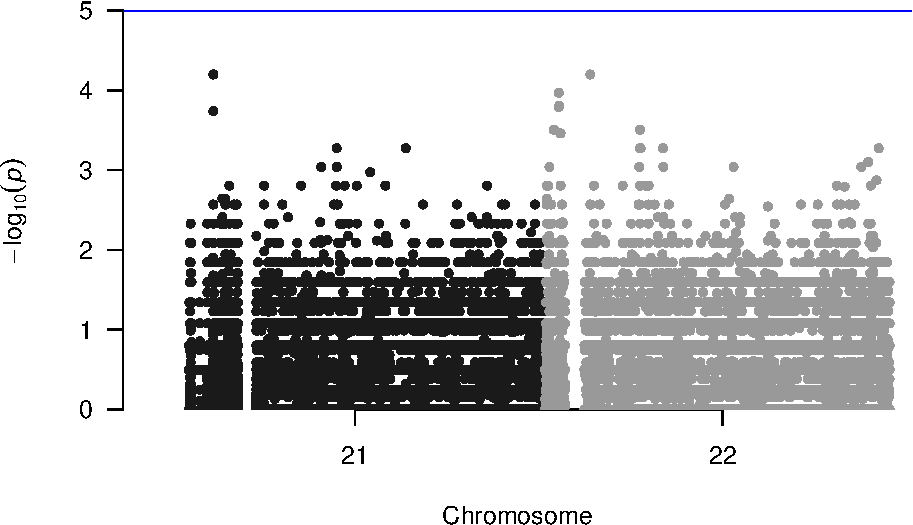
\includegraphics{GWASvisualizations_files/figure-latex/unnamed-chunk-10-1.pdf}

\begin{Shaded}
\begin{Highlighting}[]
\KeywordTok{manhattan}\NormalTok{(gwasResults)}
\end{Highlighting}
\end{Shaded}

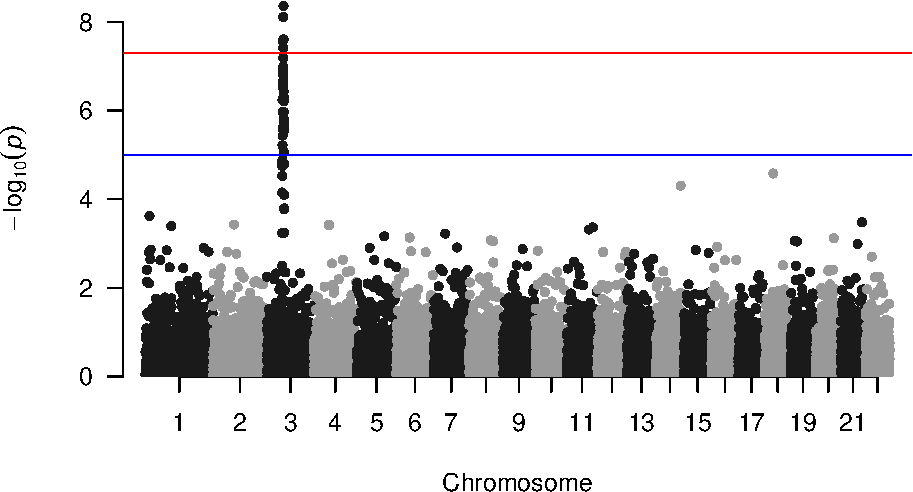
\includegraphics{GWASvisualizations_files/figure-latex/unnamed-chunk-10-2.pdf}

A list of SNP of interest is provided with the library: Let's highlight
them, with a bit of customization on the plot

\begin{Shaded}
\begin{Highlighting}[]
\KeywordTok{manhattan}\NormalTok{(final,  }\DataTypeTok{chr=}\StringTok{"CHR"}\NormalTok{, }\DataTypeTok{bp=}\StringTok{"SNP"}\NormalTok{, }\DataTypeTok{snp=}\StringTok{"dbSNP"}\NormalTok{, }\DataTypeTok{p=}\StringTok{"UNADJ"}\NormalTok{, }\DataTypeTok{highlight =} \KeywordTok{c}\NormalTok{(}\StringTok{"rs370508396"}\NormalTok{))}
\end{Highlighting}
\end{Shaded}

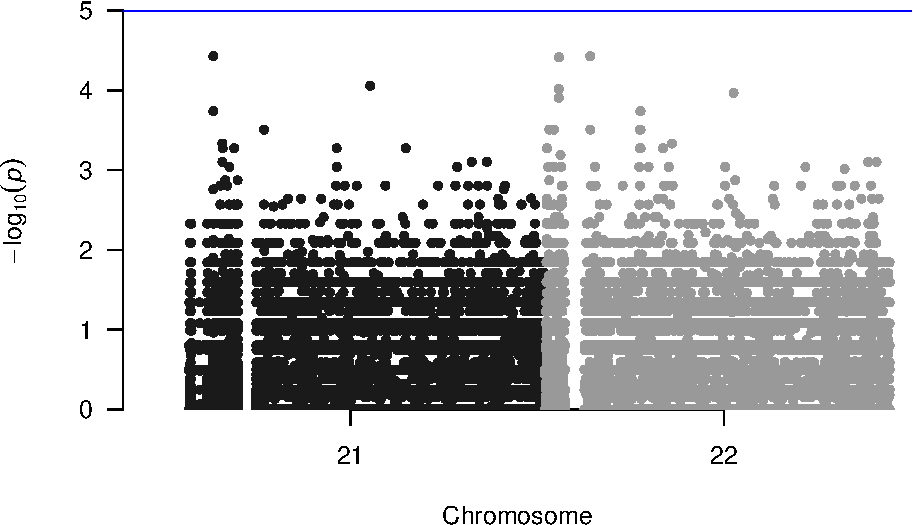
\includegraphics{GWASvisualizations_files/figure-latex/unnamed-chunk-11-1.pdf}

\begin{Shaded}
\begin{Highlighting}[]
\KeywordTok{manhattan}\NormalTok{(final,  }\DataTypeTok{chr=}\StringTok{"CHR"}\NormalTok{, }\DataTypeTok{bp=}\StringTok{"SNP"}\NormalTok{, }\DataTypeTok{snp=}\StringTok{"dbSNP"}\NormalTok{, }\DataTypeTok{p=}\StringTok{"UNADJ"}\NormalTok{, }\DataTypeTok{annotatePval =} \FloatTok{0.5}\NormalTok{)}
\end{Highlighting}
\end{Shaded}

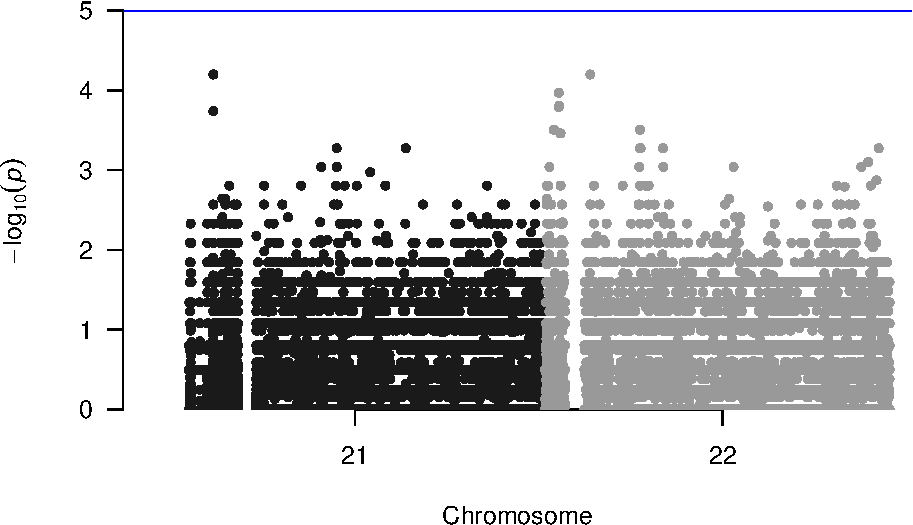
\includegraphics{GWASvisualizations_files/figure-latex/unnamed-chunk-12-1.pdf}

\begin{Shaded}
\begin{Highlighting}[]
\KeywordTok{manhattan}\NormalTok{(gwasResults, }\DataTypeTok{annotatePval =} \FloatTok{0.05}\NormalTok{)}
\end{Highlighting}
\end{Shaded}

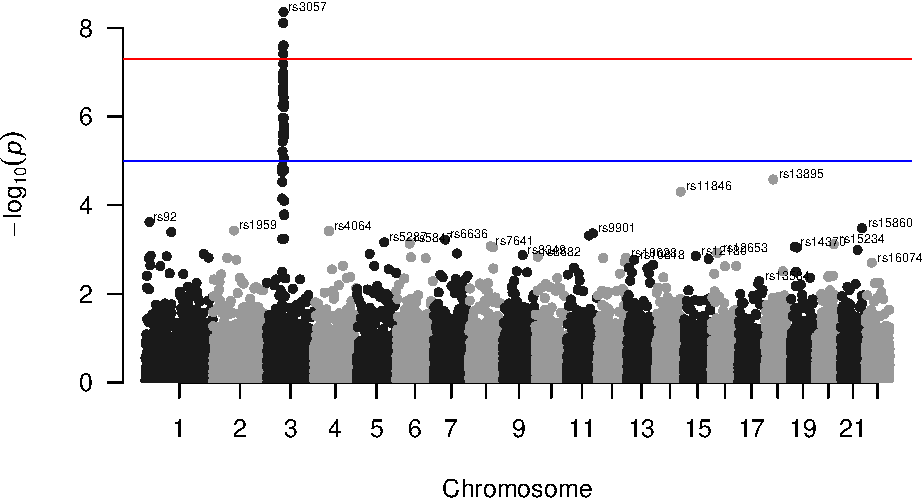
\includegraphics{GWASvisualizations_files/figure-latex/unnamed-chunk-12-2.pdf}

\hypertarget{qqplot-it-is-a-good-practice-to-draw-a-qqplot-from-the-output-of-a-gwas.-it-allows-to-compare-the-distribution-of-the-pvalue-with-an-expected-distribution-by-chance.-its-realisation-is-straightforward-thanks-to-the-qq-function}{%
\subsection{qqplot It is a good practice to draw a qqplot from the
output of a GWAS. It allows to compare the distribution of the pvalue
with an expected distribution by chance. Its realisation is
straightforward thanks to the qq
function:}\label{qqplot-it-is-a-good-practice-to-draw-a-qqplot-from-the-output-of-a-gwas.-it-allows-to-compare-the-distribution-of-the-pvalue-with-an-expected-distribution-by-chance.-its-realisation-is-straightforward-thanks-to-the-qq-function}}

\begin{Shaded}
\begin{Highlighting}[]
\KeywordTok{qq}\NormalTok{(final}\OperatorTok{$}\NormalTok{UNADJ)}
\end{Highlighting}
\end{Shaded}

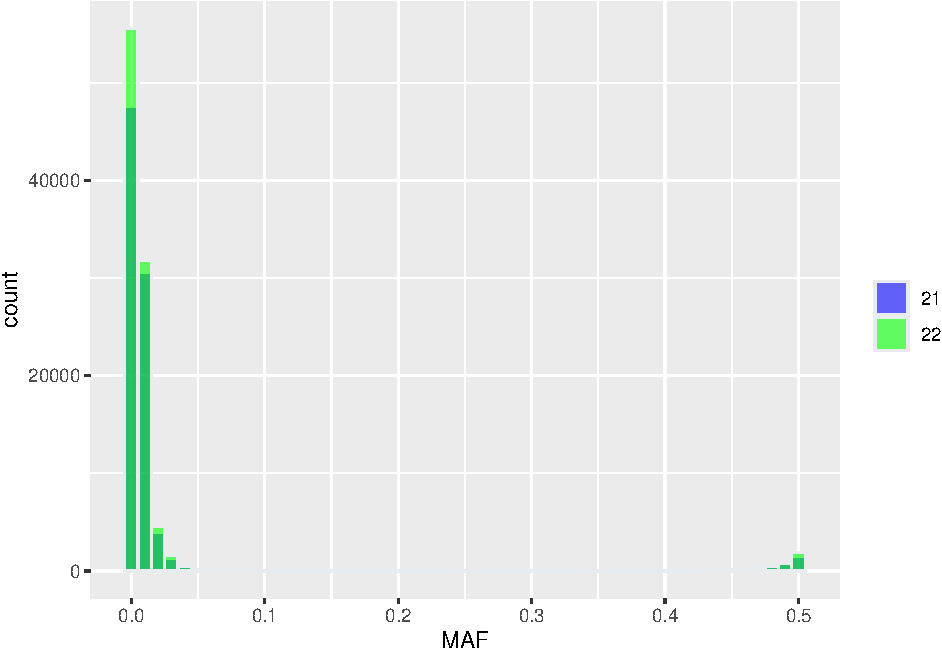
\includegraphics{GWASvisualizations_files/figure-latex/unnamed-chunk-13-1.pdf}

We have tons of other metadata, what else would be interesting to
explore?

\hypertarget{circular-version-with-cmplot}{%
\subsection{circular version with
CMplot}\label{circular-version-with-cmplot}}

The CMplot library by Lilin Yin is a good choice if you want to make a
circular version of your manhattanplot. I believe than doing a circular
version makes sense: it gives less space to all the non significant SNPs
that do not interest us, and gives more space for the significant
association. Moreover, the CMplot makes their realization
straightforward.

\begin{Shaded}
\begin{Highlighting}[]
\KeywordTok{library}\NormalTok{(}\StringTok{"CMplot"}\NormalTok{)}
\KeywordTok{CMplot}\NormalTok{(gwasResults, }\DataTypeTok{plot.type=}\StringTok{"c"}\NormalTok{, }\DataTypeTok{r=}\FloatTok{1.6}\NormalTok{, }\DataTypeTok{cir.legend=}\OtherTok{TRUE}\NormalTok{,}
        \DataTypeTok{outward=}\OtherTok{TRUE}\NormalTok{, }\DataTypeTok{cir.legend.col=}\StringTok{"black"}\NormalTok{, }\DataTypeTok{cir.chr.h=}\NormalTok{.}\DecValTok{1}\NormalTok{ ,}\DataTypeTok{chr.den.col=}\StringTok{"orange"}\NormalTok{, }\DataTypeTok{file=}\StringTok{"jpg"}\NormalTok{,}
        \DataTypeTok{memo=}\StringTok{""}\NormalTok{, }\DataTypeTok{dpi=}\DecValTok{300}\NormalTok{, }\DataTypeTok{chr.labels=}\KeywordTok{seq}\NormalTok{(}\DecValTok{1}\NormalTok{,}\DecValTok{22}\NormalTok{))}
\end{Highlighting}
\end{Shaded}

\begin{verbatim}
##  Circular-Manhattan Plotting P.
##  Plots are stored in: /Users/keithmitchell/Desktop/Repositories/2021-July-Genome-Wide-Association-Studies/data_analysis
\end{verbatim}

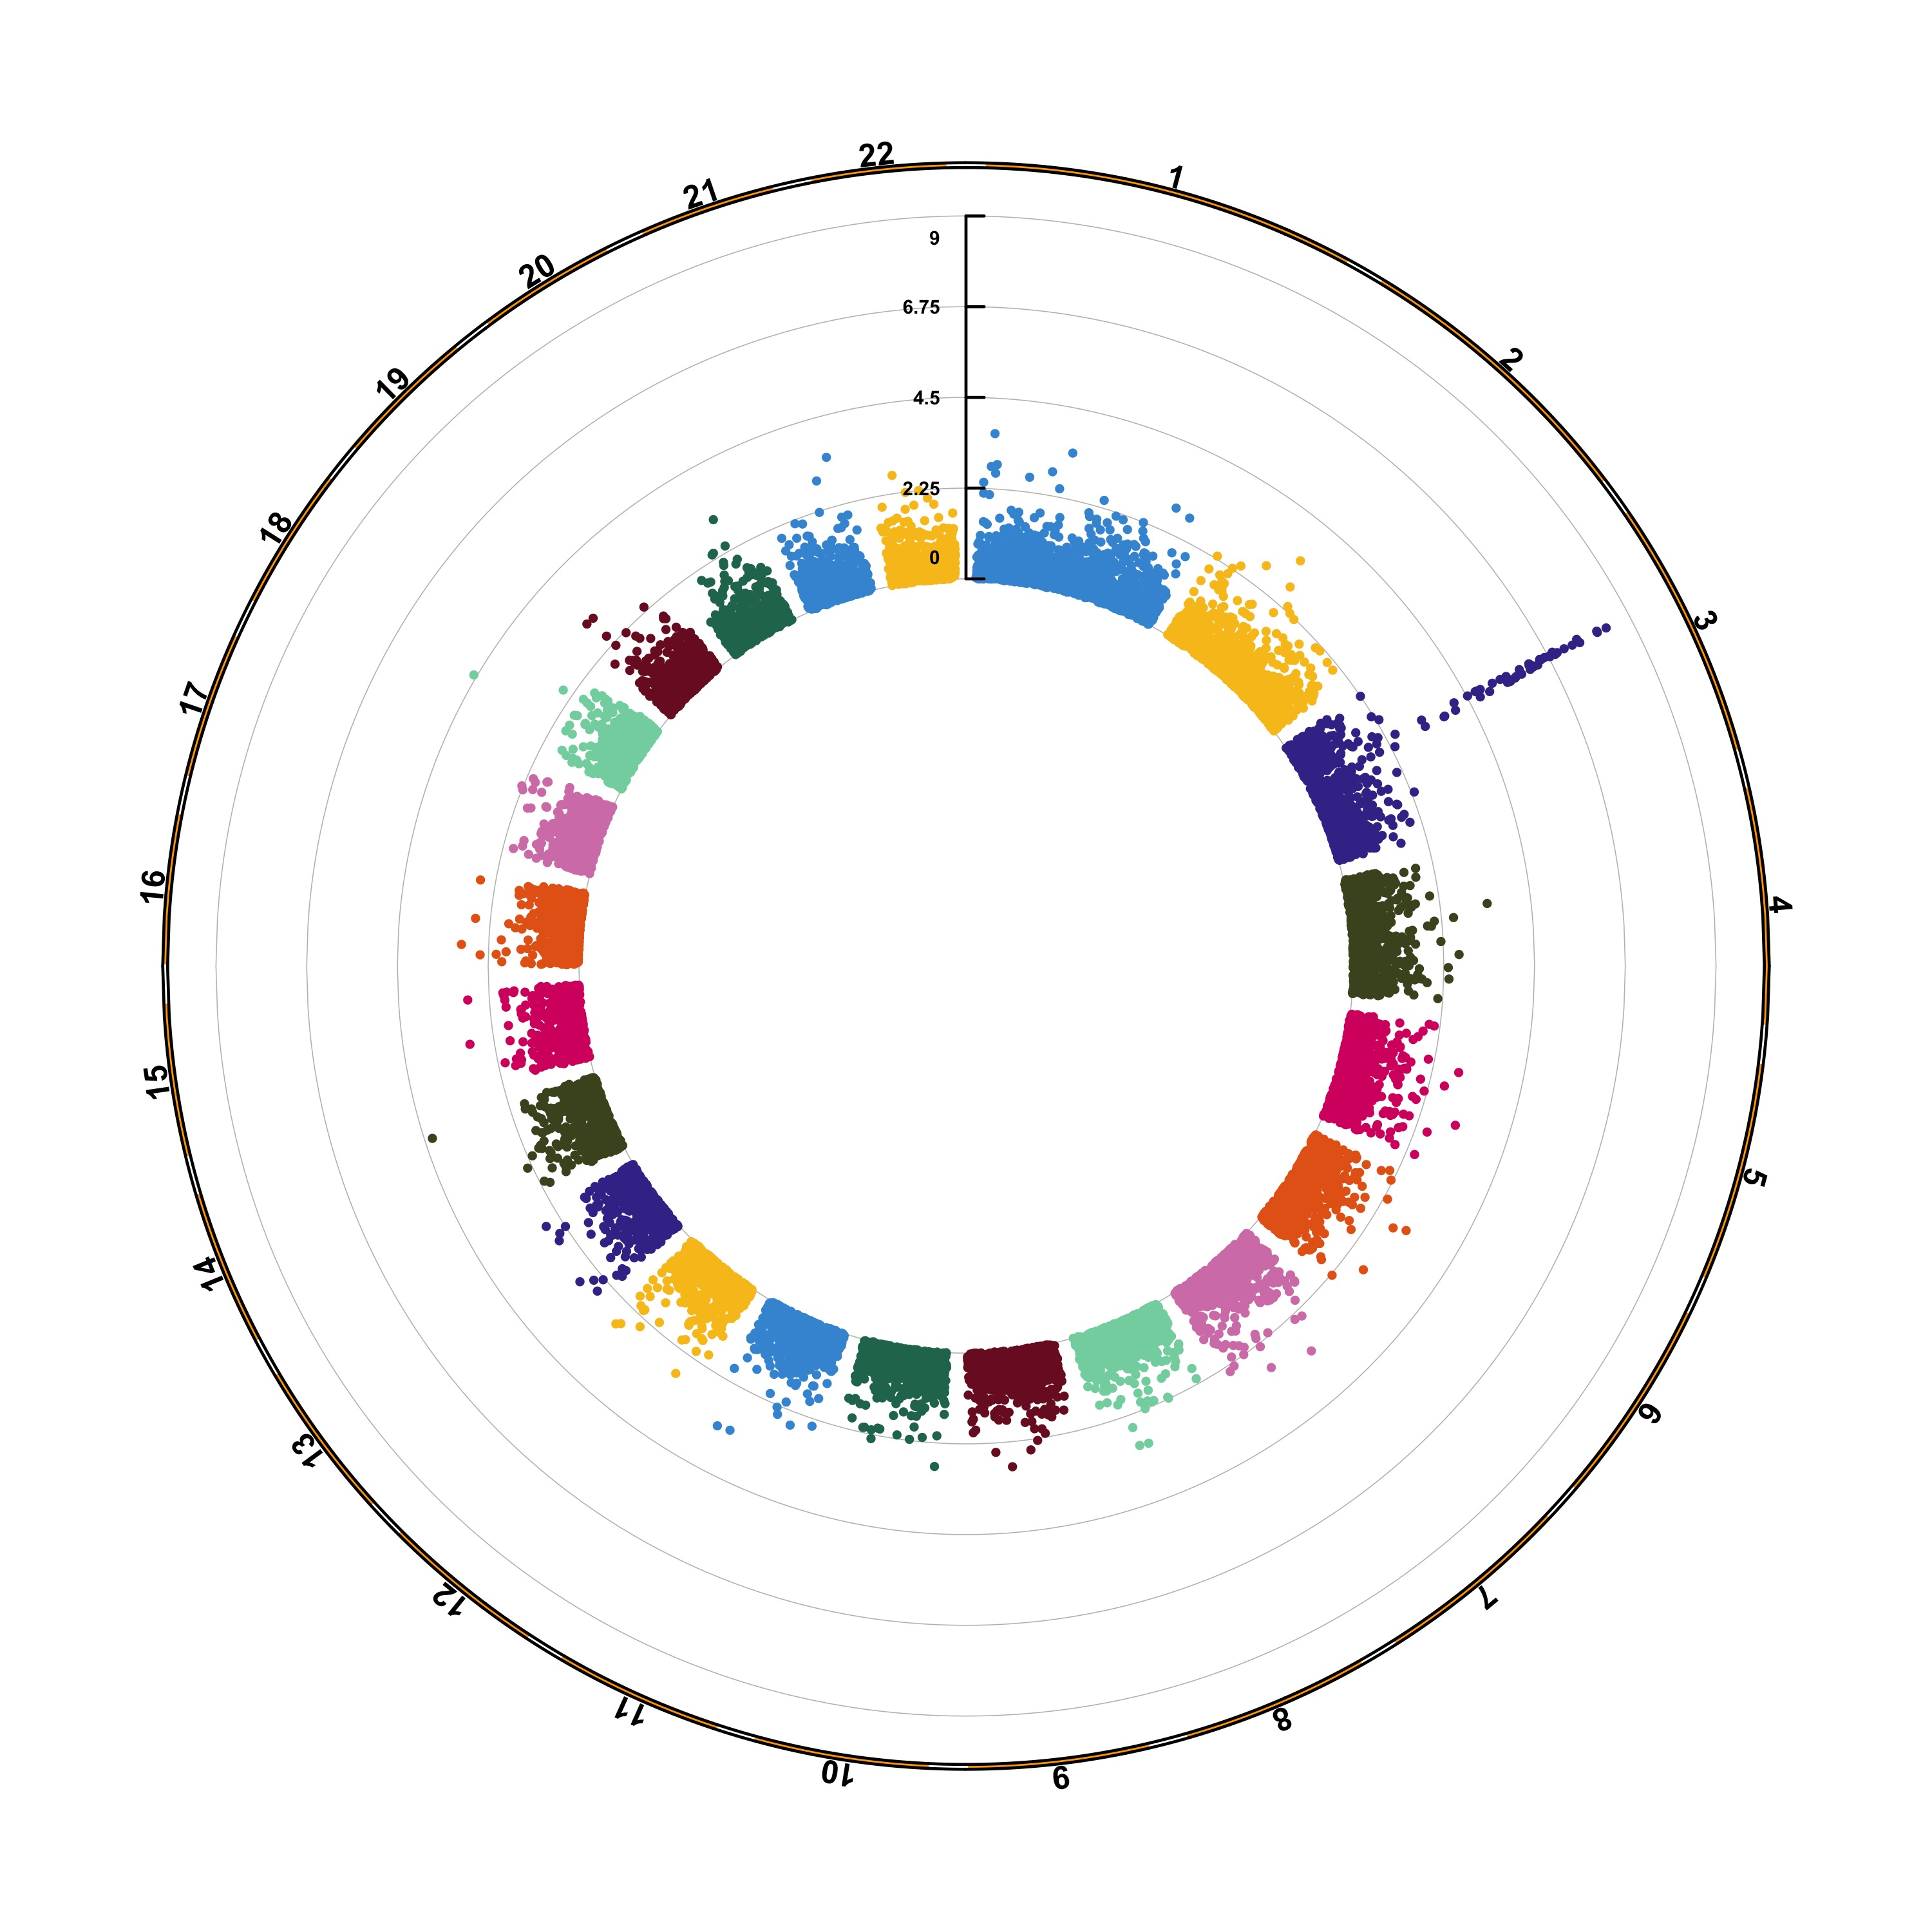
\includegraphics{../Circular-Manhattan.P.jpg}

\end{document}
